\section{Results of fits for invariant four lepton mass in data}

\begin{figure}[htbp]
\begin{center}
    \subfigure[$4e$]{
      \includegraphics[width=0.48\textwidth,angle=0]{Plots/Result_Combine_Ratio_SM_125_mass4l_floatPOIs_fixMH_fixDeltaMHmZ_all_8TeV_xs_v2_result_plot_4e_Unpublished.pdf}
    }
    \subfigure[$4\mu$]{
      \includegraphics[width=0.48\textwidth,angle=0]{Plots/Result_Combine_Ratio_SM_125_mass4l_floatPOIs_fixMH_fixDeltaMHmZ_all_8TeV_xs_v2_result_plot_4mu_Unpublished.pdf}
    } \\
    \subfigure[$2e2\mu$]{
      \includegraphics[width=0.48\textwidth,angle=0]{Plots/Result_Combine_Ratio_SM_125_mass4l_floatPOIs_fixMH_fixDeltaMHmZ_all_8TeV_xs_v2_result_plot_2e2mu_Unpublished.pdf}
    }
    \subfigure[$4\ell$]{
      \includegraphics[width=0.48\textwidth,angle=0]{Plots/Result_Combine_Ratio_SM_125_mass4l_floatPOIs_fixMH_fixDeltaMHmZ_all_8TeV_xs_v2_result_plot_4l.pdf}
    }
        \caption{Inclusive four lepton mass distributions after the simultaneous fit for $\Hllll$ and $\Zllll$ in data, and resulting fitted values of the signal and background pdfs in different final states.}
\end{center}
\end{figure}
%============

%============
\begin{figure}[htb]
  \begin{center}
    \subfigure[$0.0 \GeV < \pt(\mathrm{H}) < 15.0 \GeV$]{
      \includegraphics[width=0.45\textwidth,angle=0]{Plots/data_unfoldwith_SM_125_v3_pT4l_4l_recobin0_unpublished.pdf}
    }
    \subfigure[$15.0 \GeV < \pt(\mathrm{H}) < 30.0 \GeV$]{
      \includegraphics[width=0.45\textwidth,angle=0]{Plots/data_unfoldwith_SM_125_v3_pT4l_4l_recobin1_unpublished.pdf}
    } \\
    \subfigure[$30.0 \GeV < \pt(\mathrm{H}) < 60.0 \GeV$]{
      \includegraphics[width=0.45\textwidth,angle=0]{Plots/data_unfoldwith_SM_125_v3_pT4l_4l_recobin2_unpublished.pdf}
    }
    \subfigure[$60.0 \GeV < \pt(\mathrm{H}) < 200.0 \GeV$]{
      \includegraphics[width=0.45\textwidth,angle=0]{Plots/data_unfoldwith_SM_125_v3_pT4l_4l_recobin3_unpublished.pdf}
    } \\
    \caption{Four lepton mass distributions after the standalone fit for $\Hllll$ in data, and resulting fitted values of the signal and background pdfs in different bins of $\pt(\mathrm{H})$ (all final states combined).}
  \end{center}
\end{figure} 


%============
\begin{figure}[htb]
  \begin{center}
    \subfigure[$0.0  < |y(\mathrm{H})| < 0.4 $]{
      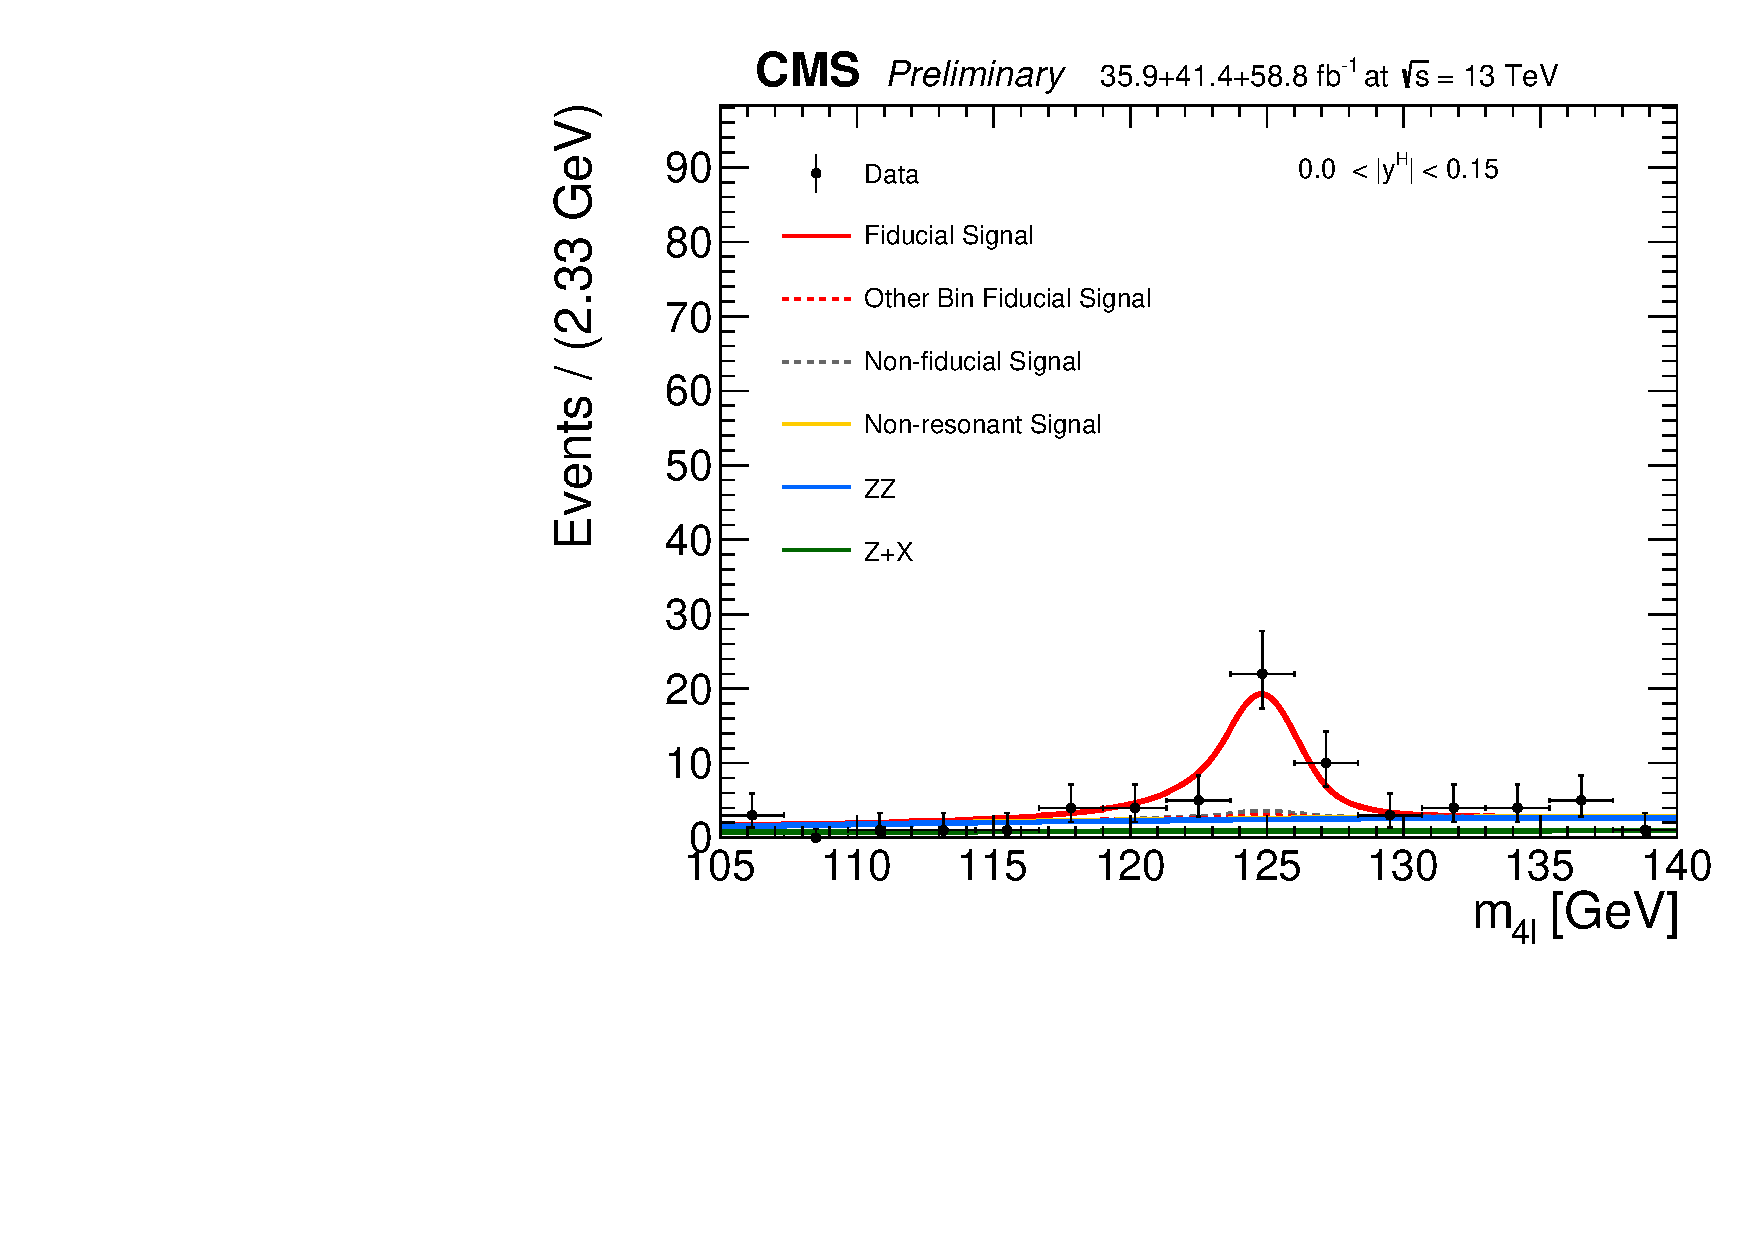
\includegraphics[width=0.45\textwidth,angle=0]{Plots/data_unfoldwith_SM_125_v3_rapidity4l_4l_recobin0.pdf}
       \label{fig:sigfits-data-rapidity4l-4l:a}
    }
    \subfigure[$0.4  < |y(\mathrm{H})| < 0.8 $]{
      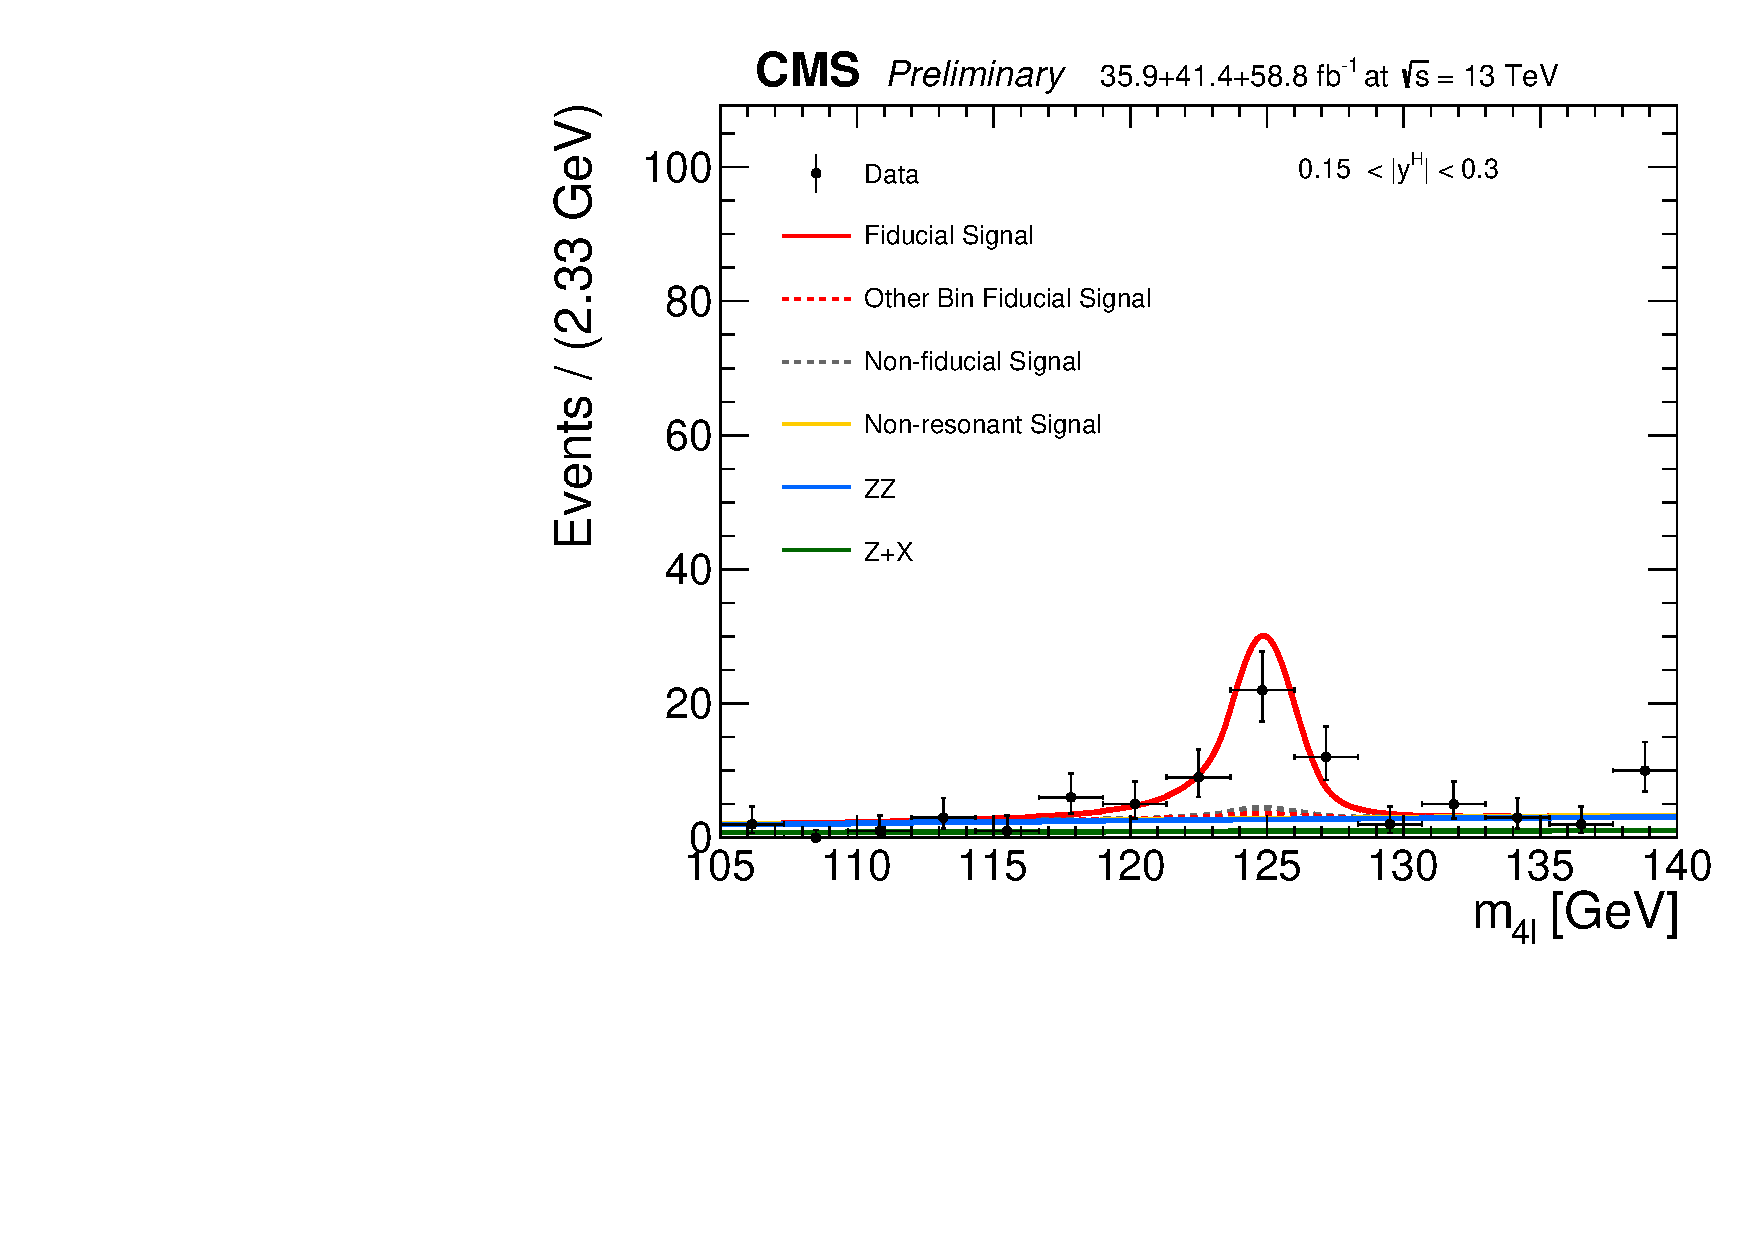
\includegraphics[width=0.45\textwidth,angle=0]{Plots/data_unfoldwith_SM_125_v3_rapidity4l_4l_recobin1.pdf}
       \label{fig:sigfits-data-rapidity4l-4l:b}
    } \\
    \subfigure[$0.8  < |y(\mathrm{H})| < 1.2 $]{
      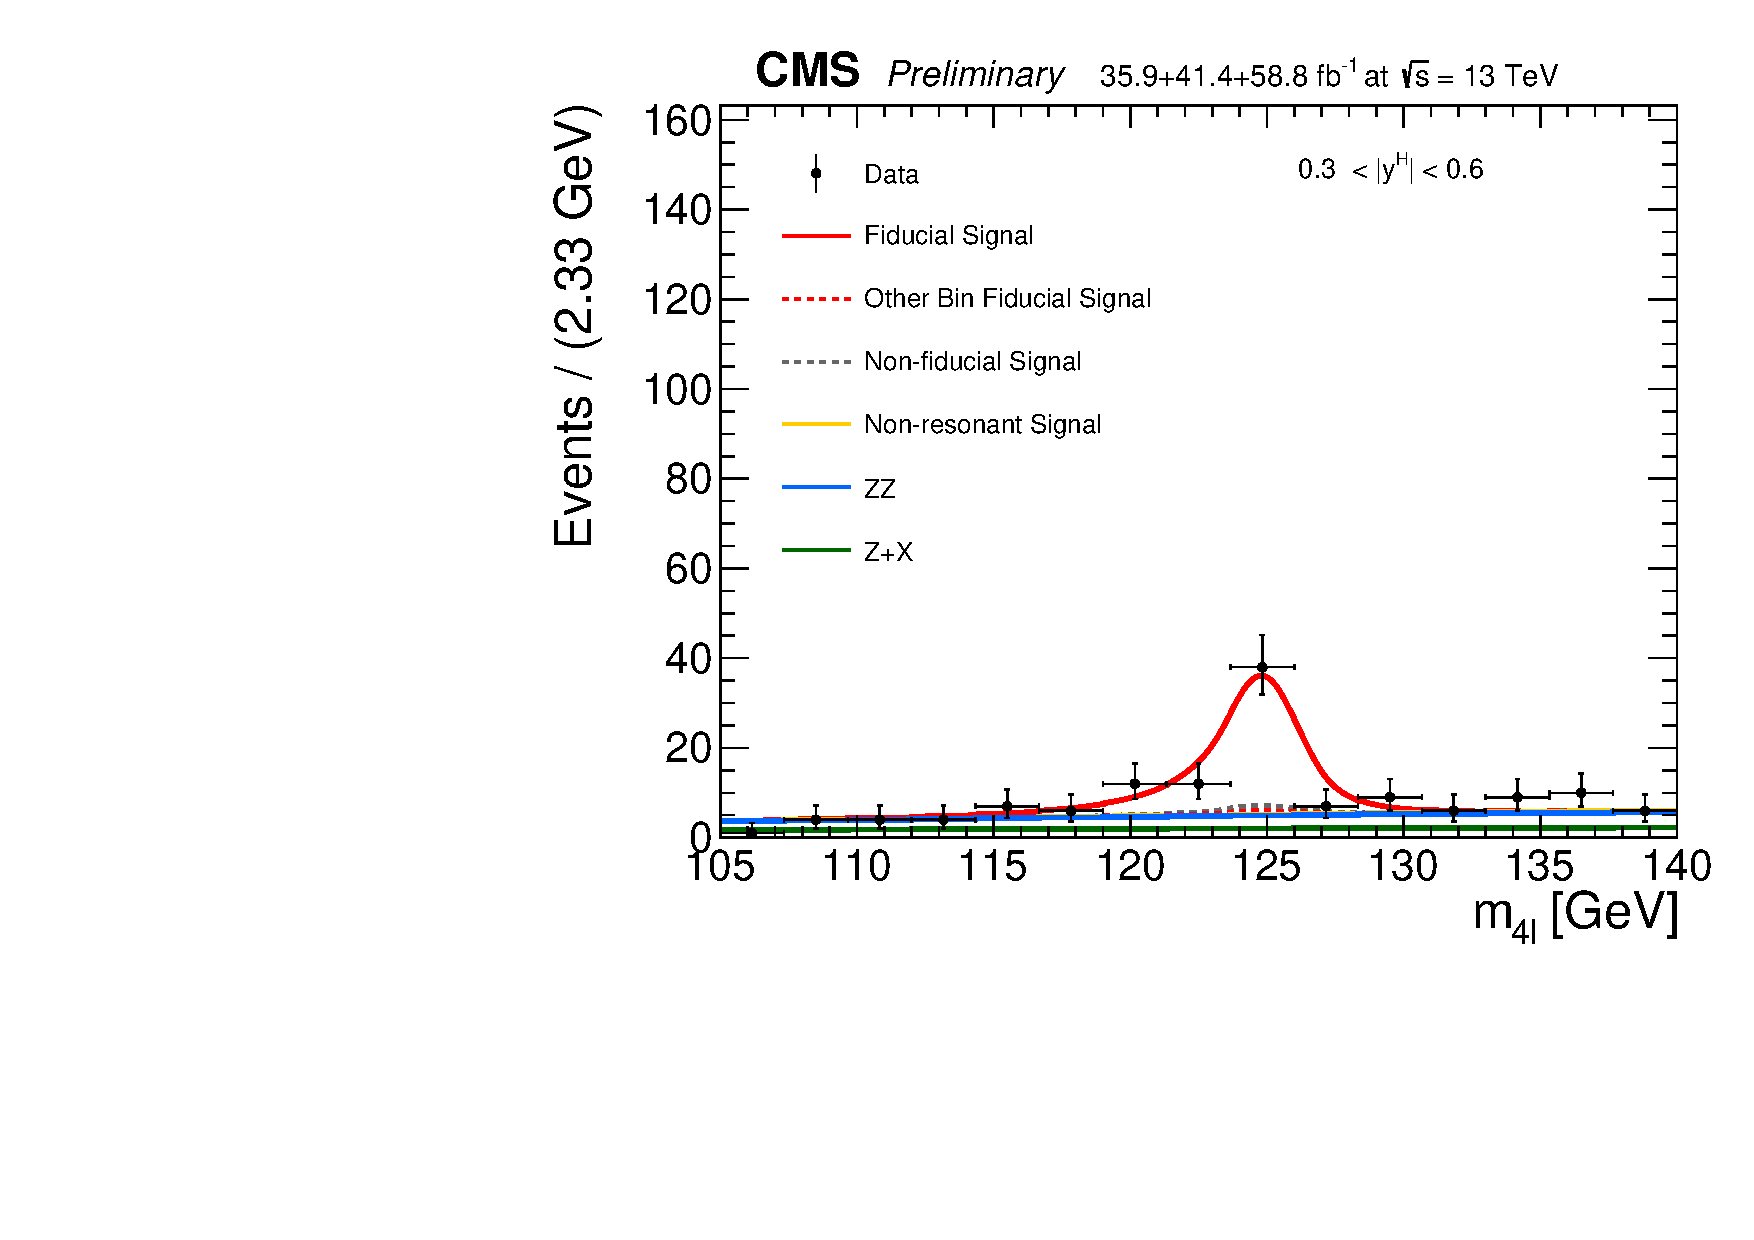
\includegraphics[width=0.45\textwidth,angle=0]{Plots/data_unfoldwith_SM_125_v3_rapidity4l_4l_recobin2.pdf}
       \label{fig:sigfits-data-rapidity4l-4l:c}
    }
    \subfigure[$1.2  < |y(\mathrm{H})| < 2.4 $]{
      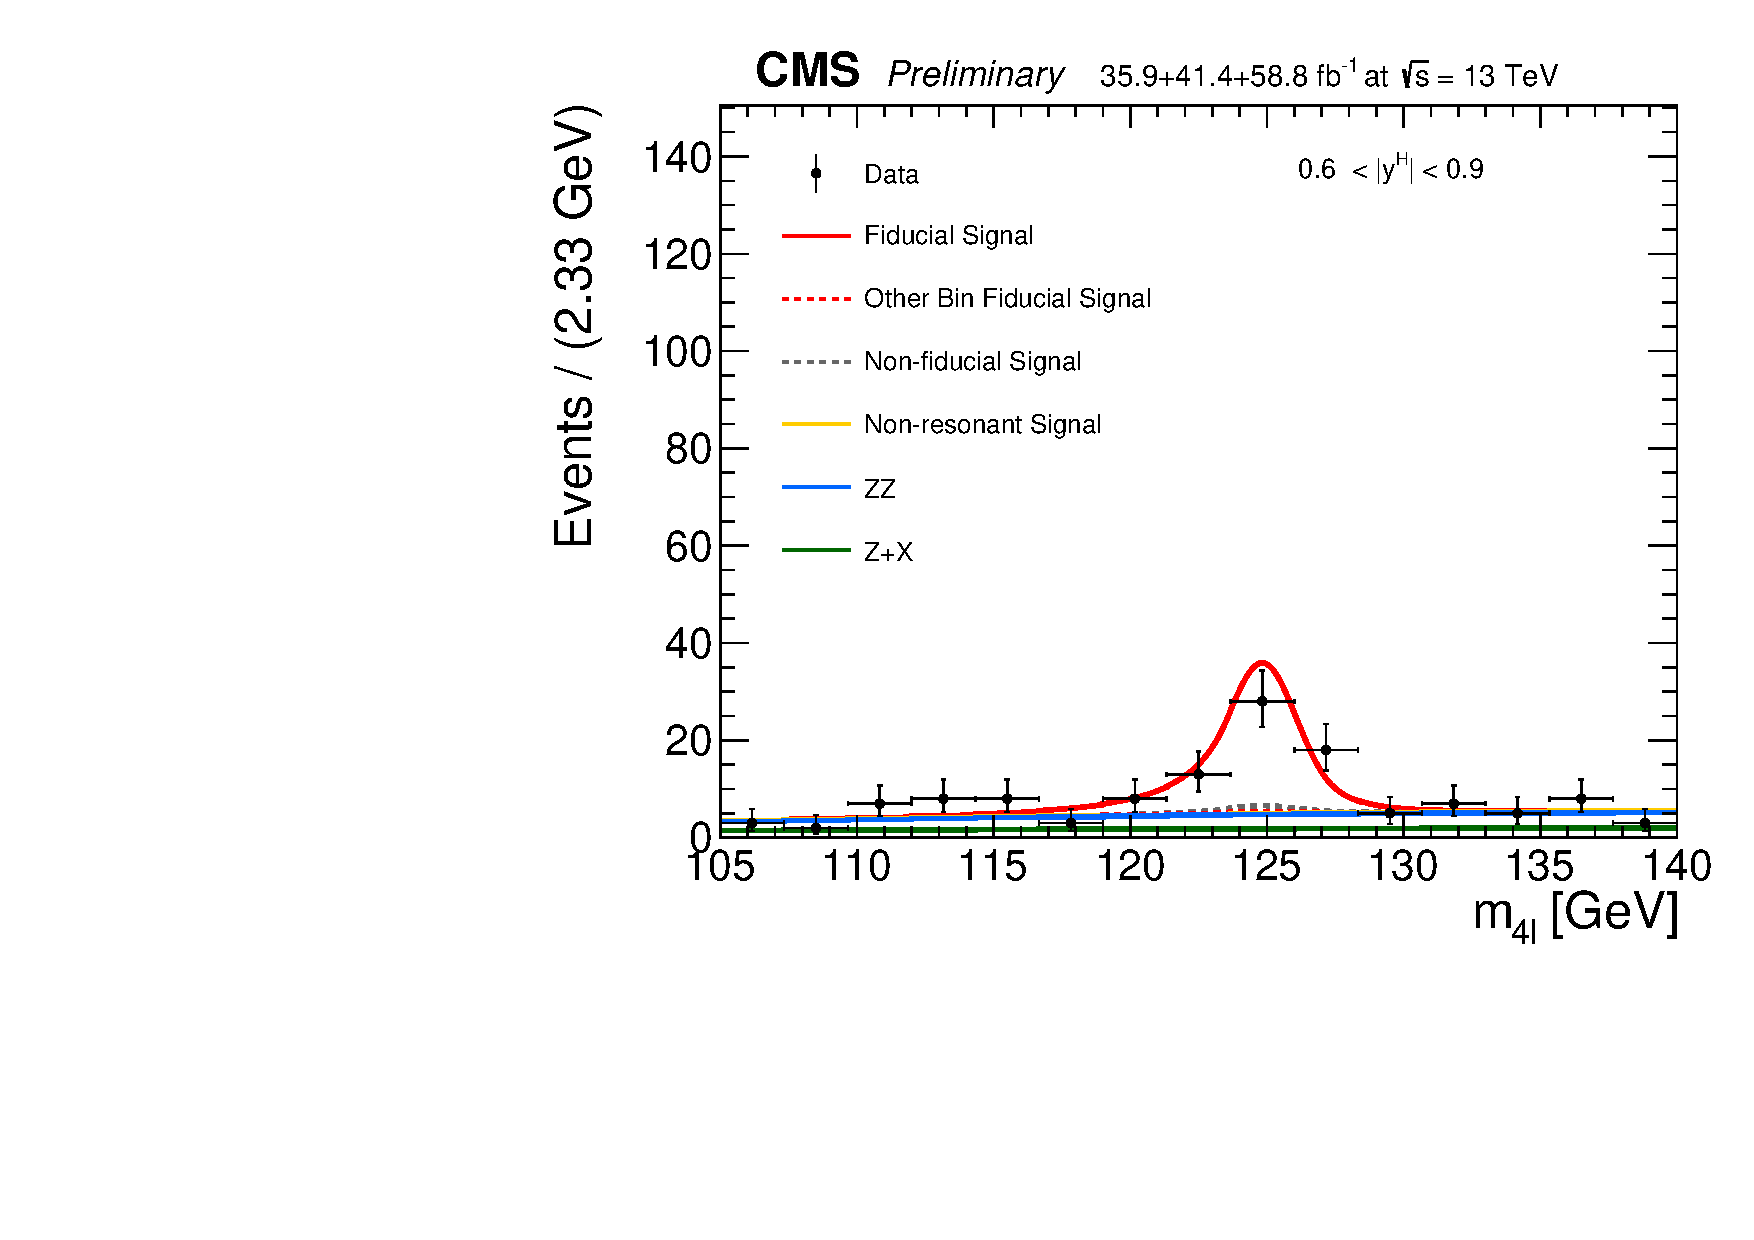
\includegraphics[width=0.45\textwidth,angle=0]{Plots/data_unfoldwith_SM_125_v3_rapidity4l_4l_recobin3.pdf}
       \label{fig:sigfits-data-rapidity4l-4l:d}
    } \\
    \caption{Four lepton mass distributions after the standalone fit for $\Hllll$ in data, and resulting fitted values of the signal and background pdfs in different bins of $y(\mathrm{H})$ (all final states combined).}
  \label{fig:sigfits-data-SM-rapidity4l-4l}
  \end{center}
\end{figure} 


%============
\begin{figure}[htb]
  \begin{center}
    \subfigure[N(jets)=0, $|\eta|<4.7$]{
      \includegraphics[width=0.45\textwidth,angle=0]{Plots/data_unfoldwith_SM_125_v3_njets_reco_pt30_eta4p7_4l_recobin0_unpublished.pdf}
       \label{fig:sigfits-data-njets_reco_pt30_eta4p7-4l:a}
    }
    \subfigure[N(jets)=1, $|\eta|<4.7$]{
      \includegraphics[width=0.45\textwidth,angle=0]{Plots/data_unfoldwith_SM_125_v3_njets_reco_pt30_eta4p7_4l_recobin1_unpublished.pdf}
       \label{fig:sigfits-data-njets_reco_pt30_eta4p7-4l:b}
    } \\
    \subfigure[N(jets)=2, $|\eta|<4.7$]{
      \includegraphics[width=0.45\textwidth,angle=0]{Plots/data_unfoldwith_SM_125_v3_njets_reco_pt30_eta4p7_4l_recobin2_unpublished.pdf}
       \label{fig:sigfits-data-njets_reco_pt30_eta4p7-4l:c}
    }
    \subfigure[N(jets) $\ge$ 3, $|\eta|<4.7$]{
      \includegraphics[width=0.45\textwidth,angle=0]{Plots/data_unfoldwith_SM_125_v3_njets_reco_pt30_eta4p7_4l_recobin3_unpublished.pdf}
       \label{fig:sigfits-data-njets_reco_pt30_eta4p7-4l:d}
    } \\
    \caption{Four lepton mass distributions after the standalone fit for $\Hllll$ in data, and resulting fitted values of the signal and background pdfs in different bins of N(jets), $|\eta|<4.7$ (all final states combined).}
  \label{fig:sigfits-data-njets_reco_pt30_eta4p7-4l}
  \end{center}
\end{figure} 


%============
\begin{figure}[htb]
  \begin{center}
    \subfigure[N(jets)=0, $|\eta|<2.5$]{
      \includegraphics[width=0.45\textwidth,angle=0]{Plots/data_unfoldwith_SM_125_v3_njets_reco_pt30_eta2p5_4l_recobin0.pdf}
       \label{fig:sigfits-data-njets_reco_pt30_eta2p5-4l:a}
    }
    \subfigure[N(jets)=1, $|\eta|<2.5$]{
      \includegraphics[width=0.45\textwidth,angle=0]{Plots/data_unfoldwith_SM_125_v3_njets_reco_pt30_eta2p5_4l_recobin1.pdf}
       \label{fig:sigfits-data-njets_reco_pt30_eta2p5-4l:b}
    } \\
    \subfigure[N(jets)=2, $|\eta|<2.5$]{
      \includegraphics[width=0.45\textwidth,angle=0]{Plots/data_unfoldwith_SM_125_v3_njets_reco_pt30_eta2p5_4l_recobin2.pdf}
       \label{fig:sigfits-data-njets_reco_pt30_eta2p5-4l:c}
    }
    \subfigure[N(jets) $\ge$ 3, $|\eta|<2.5$]{
      \includegraphics[width=0.45\textwidth,angle=0]{Plots/data_unfoldwith_SM_125_v3_njets_reco_pt30_eta2p5_4l_recobin3.pdf}
       \label{fig:sigfits-data-njets_reco_pt30_eta2p5-4l:d}
    } \\
    \caption{Four lepton mass distributions after the standalone fit for $\Hllll$ in data, and resulting fitted values of the signal and background pdfs in different bins of N(jets), $|\eta|<2.5$ (all final states combined).}
  \label{fig:sigfits-data-njets_reco_pt30_eta2p5-4l}
  \end{center}
\end{figure} 



%============
\begin{figure}[htb]
  \begin{center}
    \subfigure[$40.0 \GeV < {\rm m}({\rm Z}_{1}) < 75.0 \GeV$]{
      \includegraphics[width=0.45\textwidth,angle=0]{Plots/data_unfoldwith_SM_125_v3_massZ1_4l_recobin0.pdf}
       \label{fig:sigfits-data-massZ1-4l:a}
    }
    \subfigure[$75.0 \GeV <{\rm m}({\rm Z}_{1}) < 87.2 \GeV$]{
      \includegraphics[width=0.45\textwidth,angle=0]{Plots/data_unfoldwith_SM_125_v3_massZ1_4l_recobin1.pdf}
       \label{fig:sigfits-data-massZ1-4l:b}
    } \\
    \subfigure[$87.2 \GeV <{\rm m}({\rm Z}_{1}) < 95.2 \GeV$]{
      \includegraphics[width=0.45\textwidth,angle=0]{Plots/data_unfoldwith_SM_125_v3_massZ1_4l_recobin2.pdf}
       \label{fig:sigfits-data-massZ1-4l:c}
    }
    \subfigure[$95.2 \GeV <{\rm m}({\rm Z}_{1}) < 120.0 \GeV$]{
      \includegraphics[width=0.45\textwidth,angle=0]{Plots/data_unfoldwith_SM_125_v3_massZ1_4l_recobin3.pdf}
       \label{fig:sigfits-data-massZ1-4l:d}
    } \\
    \caption{Four lepton mass distributions after the standalone fit for $\Hllll$ in data, and resulting fitted values of the signal and background pdfs in different bins of ${\rm m}({\rm Z}_{1})$ (all final states combined).}
  \label{fig:sigfits-data-massZ1-4l}
  \end{center}
\end{figure} 


%============
\begin{figure}[htb]
  \begin{center}
    \subfigure[$12.0 \GeV < {\rm m}({\rm Z}_{2}) < 20.0 \GeV$]{
      \includegraphics[width=0.45\textwidth,angle=0]{Plots/data_unfoldwith_SM_125_v3_massZ2_4l_recobin0.pdf}
       \label{fig:sigfits-data-massZ2-4l:a}
    }
    \subfigure[$20.0 \GeV <{\rm m}({\rm Z}_{2}) < 28.0 \GeV$]{
      \includegraphics[width=0.45\textwidth,angle=0]{Plots/data_unfoldwith_SM_125_v3_massZ2_4l_recobin1.pdf}
       \label{fig:sigfits-data-massZ2-4l:b}
    } \\
    \subfigure[$28.0 \GeV <{\rm m}({\rm Z}_{2}) < 35.0 \GeV$]{
      \includegraphics[width=0.45\textwidth,angle=0]{Plots/data_unfoldwith_SM_125_v3_massZ2_4l_recobin2.pdf}
       \label{fig:sigfits-data-massZ2-4l:c}
    }
    \subfigure[$35.0 \GeV <{\rm m}({\rm Z}_{2}) < 60.0 \GeV$]{
      \includegraphics[width=0.45\textwidth,angle=0]{Plots/data_unfoldwith_SM_125_v3_massZ2_4l_recobin3.pdf}
       \label{fig:sigfits-data-massZ2-4l:d}
    } \\
    \caption{Four lepton mass distributions after the standalone fit for $\Hllll$ in data, and resulting fitted values of the signal and background pdfs in different bins of ${\rm m}({\rm Z}_{2})$ (all final states combined).}
  \label{fig:sigfits-data-massZ2-4l}
  \end{center}
\end{figure} 

%============
\begin{figure}[htb]
  \begin{center}
    \subfigure[$0.0  < |\cos \theta^{*}| < 0.25 $]{
      \includegraphics[width=0.45\textwidth,angle=0]{Plots/data_unfoldwith_SM_125_v3_cosThetaStar_4l_recobin0.pdf}
       \label{fig:sigfits-data-cosThetaStar-4l:a}
    }
    \subfigure[$0.25  < |\cos \theta^{*}| < 0.5 $]{
      \includegraphics[width=0.45\textwidth,angle=0]{Plots/data_unfoldwith_SM_125_v3_cosThetaStar_4l_recobin1.pdf}
       \label{fig:sigfits-data-cosThetaStar-4l:b}
    } \\
    \subfigure[$0.5  < |\cos \theta^{*}| < 0.75 $]{
      \includegraphics[width=0.45\textwidth,angle=0]{Plots/data_unfoldwith_SM_125_v3_cosThetaStar_4l_recobin2.pdf}
       \label{fig:sigfits-data-cosThetaStar-4l:c}
    }
    \subfigure[$0.75  < |\cos \theta^{*}| < 1.0 $]{
      \includegraphics[width=0.45\textwidth,angle=0]{Plots/data_unfoldwith_SM_125_v3_cosThetaStar_4l_recobin3.pdf}
       \label{fig:sigfits-data-cosThetaStar-4l:d}
    } \\
    \caption{Four lepton mass distributions after the standalone fit for $\Hllll$ in data, and resulting fitted values of the signal and background pdfs in different bins of $|\cos \theta^{*}|$ (all final states combined).}
  \label{fig:sigfits-data-cosThetaStar-4l}
  \end{center}
\end{figure} 

%============
\begin{figure}[htb]
  \begin{center}
    \subfigure[$0.0  < |\cos \theta_{1}| < 0.25 $]{
      \includegraphics[width=0.45\textwidth,angle=0]{Plots/data_unfoldwith_SM_125_v3_cosTheta1_4l_recobin0.pdf}
       \label{fig:sigfits-data-cosTheta1-4l:a}
    }
    \subfigure[$0.25  < |\cos \theta_{1}| < 0.5 $]{
      \includegraphics[width=0.45\textwidth,angle=0]{Plots/data_unfoldwith_SM_125_v3_cosTheta1_4l_recobin1.pdf}
       \label{fig:sigfits-data-cosTheta1-4l:b}
    } \\
    \subfigure[$0.5  < |\cos \theta_{1}| < 0.75 $]{
      \includegraphics[width=0.45\textwidth,angle=0]{Plots/data_unfoldwith_SM_125_v3_cosTheta1_4l_recobin2.pdf}
       \label{fig:sigfits-data-cosTheta1-4l:c}
    }
    \subfigure[$0.75  < |\cos \theta_{1}| < 1.0 $]{
      \includegraphics[width=0.45\textwidth,angle=0]{Plots/data_unfoldwith_SM_125_v3_cosTheta1_4l_recobin3.pdf}
       \label{fig:sigfits-data-cosTheta1-4l:d}
    } \\
    \caption{Four lepton mass distributions after the standalone fit for $\Hllll$ in data, and resulting fitted values of the signal and background pdfs in different bins of $|\cos \theta_{1}|$ (all final states combined).}
  \label{fig:sigfits-data-cosTheta1-4l}
  \end{center}
\end{figure} 


%============
\begin{figure}[htb]
  \begin{center}
    \subfigure[$0.0  < |\cos \theta_{2}| < 0.25 $]{
      \includegraphics[width=0.45\textwidth,angle=0]{Plots/data_unfoldwith_SM_125_v3_cosTheta2_4l_recobin0.pdf}
       \label{fig:sigfits-data-cosTheta2-4l:a}
    }
    \subfigure[$0.25  < |\cos \theta_{2}| < 0.5 $]{
      \includegraphics[width=0.45\textwidth,angle=0]{Plots/data_unfoldwith_SM_125_v3_cosTheta2_4l_recobin1.pdf}
       \label{fig:sigfits-data-cosTheta2-4l:b}
    } \\
    \subfigure[$0.5  < |\cos \theta_{2}| < 0.75 $]{
      \includegraphics[width=0.45\textwidth,angle=0]{Plots/data_unfoldwith_SM_125_v3_cosTheta2_4l_recobin2.pdf}
       \label{fig:sigfits-data-cosTheta2-4l:c}
    }
    \subfigure[$0.75  < |\cos \theta_{2}| < 1.0 $]{
      \includegraphics[width=0.45\textwidth,angle=0]{Plots/data_unfoldwith_SM_125_v3_cosTheta2_4l_recobin3.pdf}
       \label{fig:sigfits-data-cosTheta2-4l:d}
    } \\
    \caption{Four lepton mass distributions after the standalone fit for $\Hllll$ in data, and resulting fitted values of the signal and background pdfs in different bins of $|\cos \theta_{2}|$ (all final states combined).}
  \label{fig:sigfits-data-cosTheta2-4l}
  \end{center}
\end{figure} 


%============
\begin{figure}[htb]
  \begin{center}
    \subfigure[$0.0  < |\Phi_{1}| < 0.78 $]{
      \includegraphics[width=0.45\textwidth,angle=0]{Plots/data_unfoldwith_SM_125_v3_Phi1_4l_recobin0.pdf}
       \label{fig:sigfits-data-Phi1-4l:a}
    }
    \subfigure[$0.78  < |\Phi_{1}| < 1.57 $]{
      \includegraphics[width=0.45\textwidth,angle=0]{Plots/data_unfoldwith_SM_125_v3_Phi1_4l_recobin1.pdf}
       \label{fig:sigfits-data-Phi1-4l:b}
    } \\
    \subfigure[$1.57  < |\Phi_{1}| < 2.35 $]{
      \includegraphics[width=0.45\textwidth,angle=0]{Plots/data_unfoldwith_SM_125_v3_Phi1_4l_recobin2.pdf}
       \label{fig:sigfits-data-Phi1-4l:c}
    }
    \subfigure[$2.35  < |\Phi_{1}| < 3.14 $]{
      \includegraphics[width=0.45\textwidth,angle=0]{Plots/data_unfoldwith_SM_125_v3_Phi1_4l_recobin3.pdf}
       \label{fig:sigfits-data-Phi1-4l:d}
    } \\
    \caption{Four lepton mass distributions after the standalone fit for $\Hllll$ in data, and resulting fitted values of the signal and background pdfs in different bins of $|\Phi_{1}|$ (all final states combined).}
  \label{fig:sigfits-data-Phi1-4l}
  \end{center}
\end{figure} 


%============
\begin{figure}[htb]
  \begin{center}
    \subfigure[$0.0  < |\Phi| < 0.78 $]{
      \includegraphics[width=0.45\textwidth,angle=0]{Plots/data_unfoldwith_SM_125_v3_Phi_4l_recobin0.pdf}
       \label{fig:sigfits-data-Phi-4l:a}
    }
    \subfigure[$0.78  < |\Phi| < 1.57 $]{
      \includegraphics[width=0.45\textwidth,angle=0]{Plots/data_unfoldwith_SM_125_v3_Phi_4l_recobin1.pdf}
       \label{fig:sigfits-data-Phi-4l:b}
    } \\
    \subfigure[$1.57  < |\Phi| < 2.35 $]{
      \includegraphics[width=0.45\textwidth,angle=0]{Plots/data_unfoldwith_SM_125_v3_Phi_4l_recobin2.pdf}
       \label{fig:sigfits-data-Phi-4l:c}
    }
    \subfigure[$2.35  < |\Phi| < 3.14 $]{
      \includegraphics[width=0.45\textwidth,angle=0]{Plots/data_unfoldwith_SM_125_v3_Phi_4l_recobin3.pdf}
       \label{fig:sigfits-data-Phi-4l:d}
    } \\
    \caption{Four lepton mass distributions after the standalone fit for $\Hllll$ in data, and resulting fitted values of the signal and background pdfs in different bins of $|\Phi|$ (all final states combined).}
  \label{fig:sigfits-data-Phi-4l}
  \end{center}
\end{figure} 




%============
\begin{figure}[htb]
  \begin{center}
    \subfigure[$4e$]{
    
      \includegraphics[width=0.48\textwidth,angle=0]{Plots/realdata_unfoldwith_SM_125_v2_mass4l_4e_recobin0_7TeV.pdf}
    }
    \subfigure[$4\mu$]{
      \includegraphics[width=0.48\textwidth,angle=0]{Plots/realdata_unfoldwith_SM_125_v2_mass4l_4mu_recobin0_7TeV.pdf}
    } \\
    \subfigure[$2e2\mu$]{
      \includegraphics[width=0.48\textwidth,angle=0]{Plots/realdata_unfoldwith_SM_125_v2_mass4l_2e2mu_recobin0_7TeV.pdf}
    }
    \subfigure[$4\ell$]{
      \includegraphics[width=0.48\textwidth,angle=0]{Plots/realdata_unfoldwith_SM_125_v2_mass4l_4l_recobin0_7TeV.pdf}
    }
    \caption{Four lepton mass distributions after the standalone fit for $\Hllll$ in 7~TeV data.}
  \label{fig:inclusive-7TeV-fits}
  \end{center}
\end{figure} 


